\documentclass{article}
\usepackage{graphicx} % Required for inserting images
\usepackage{minted}

\title{Circuitos Digitais I - Atividades 1-3: Aula 1}
\author{Luis Felipe Ferreira Soares}
\date{Outubro 2025}

\begin{document}

\maketitle

\section*{Atividade 1}
\setcounter{section}{1}

\subsection{Mux RTL/Fluxo de dados}
\begin{minted}{verilog}
module mux (
    input [1:0] D,
    input sel,
    output y
);

assign y = (D[0] & !sel) | (D[1] & sel);

endmodule
\end{minted}

\subsection{Mux Comportamental}
\begin{minted}{verilog}
module mux (
  input [1:0] D,
  input sel,
  output y
);

reg y_reg;

always @(*)
begin
  if (sel == 0)
    y_reg = D[0];
  else
    y_reg = D[1];
end

assign y = y_reg;

endmodule
\end{minted}

\subsection{Mux Estrutural}
\begin{minted}{verilog}
module mux (D, sel, y);
input [1:0] D;
input sel;
output y;

wire w1, w2, nsel;

not N1(nsel, sel);
and A1(w1, D[0], nsel);
and A2(w2, D[1], sel);
or O1(y, w1, w2);

endmodule
\end{minted}

\subsection{Testbench}
\begin{minted}{verilog}
`timescale 1ns/1ps

module mux_tb;
reg [1:0] D;
reg sel;
wire y;

mux dut (.D(D), .sel(sel), .y(y));

always #1 D[0] = !D[0];
always #2 D[1] = !D[1];
always #4 sel = !sel;

initial begin
    $display("sel | D[1] | D[0] | y");
    $monitor("%3d | %4d | %4d | %b", sel, D[1], D[0], y);
    sel = 1'b0;
    D = 2'd0;
    #8 $finish;
end

endmodule
\end{minted}

\newpage
\subsection{Console output}
\begin{verbatim}
sel | D[1] | D[0] | y
  0 |    0 |    0 | 0
  0 |    0 |    1 | 1
  0 |    1 |    0 | 0
  0 |    1 |    1 | 1
  1 |    0 |    0 | 0
  1 |    0 |    1 | 0
  1 |    1 |    0 | 1
  1 |    1 |    1 | 1
\end{verbatim}

\subsection{Mux - Portas lógicas}
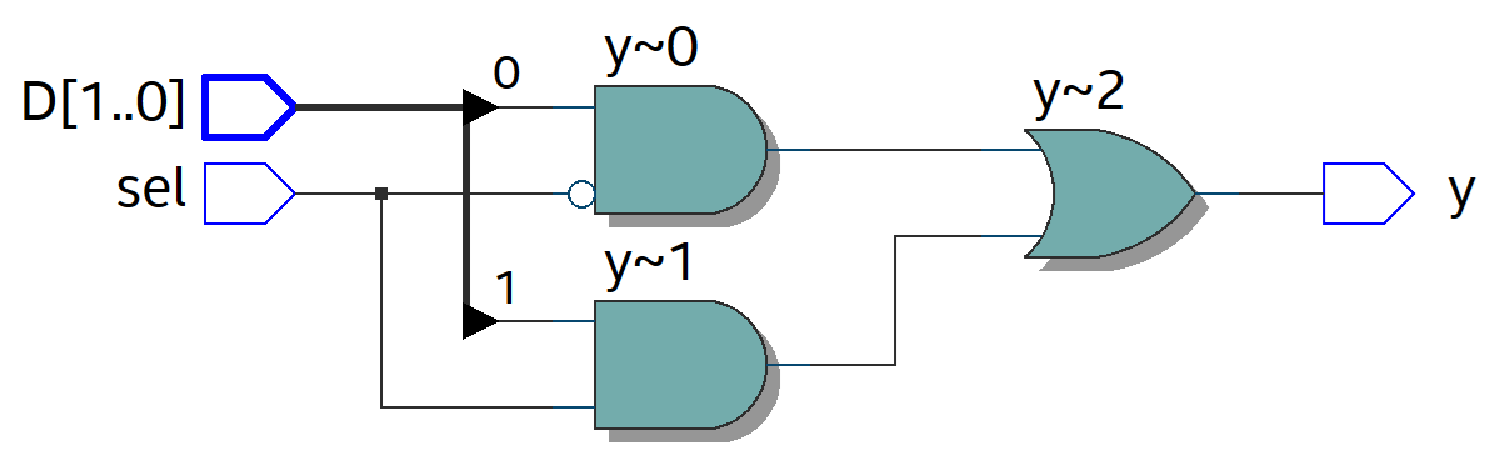
\includegraphics[width=1.0\textwidth]{mux_rtl.png}

\subsection{Mux - Simulação}
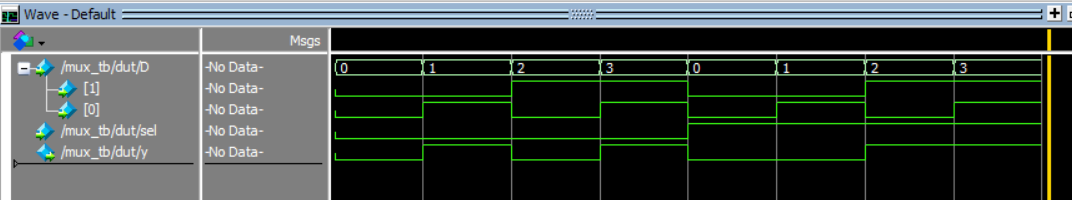
\includegraphics[width=1.0\textwidth]{mux_wave.png}

\newpage

\section*{Atividade 2}
\setcounter{section}{2}
\setcounter{subsection}{0}

\subsection{Comparador - RTL/Fluxo de dados}
\begin{minted}{verilog}
module comparador2bits (
    input [1:0] a, b,
    output y
);

assign y = !(a^b);

endmodule
\end{minted}

\subsection{Testbench}
\begin{minted}{verilog}
module comparador_tb;
reg [1:0] a, b;
wire y;

comparador2bits dut(.a(a), .b(b), .y(y));

always #1 b[0] = !b[0];
always #2 b[1] = !b[1];
always #4 a[0] = !a[0];
always #8 a[1] = !a[1];

initial begin
    $display("a[1] | a[0] | b[1] | b[0] | y");
    $monitor("%4d | %4d | %4d | %4d | %b", a[1], a[0], b[1], b[0], y);
    a = 2'b00;
    b = 2'b00;
    #16 $finish;
end

endmodule
\end{minted}

\newpage

\subsection{Console output}
\begin{verbatim}
a[1] | a[0] | b[1] | b[0] | y
   0 |    0 |    0 |    0 | 1
   0 |    0 |    0 |    1 | 0
   0 |    0 |    1 |    0 | 0
   0 |    0 |    1 |    1 | 0
   0 |    1 |    0 |    0 | 0
   0 |    1 |    0 |    1 | 1
   0 |    1 |    1 |    0 | 0
   0 |    1 |    1 |    1 | 0
   1 |    0 |    0 |    0 | 0
   1 |    0 |    0 |    1 | 0
   1 |    0 |    1 |    0 | 1
   1 |    0 |    1 |    1 | 0
   1 |    1 |    0 |    0 | 0
   1 |    1 |    0 |    1 | 0
   1 |    1 |    1 |    0 | 0
   1 |    1 |    1 |    1 | 1
\end{verbatim}

\subsection{Comparador - Portas lógicas}
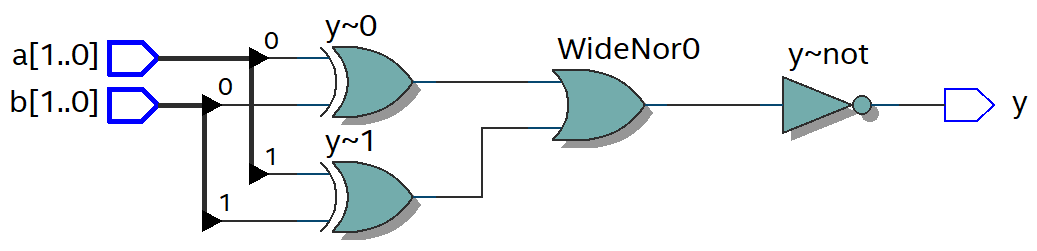
\includegraphics[width=1.0\textwidth]{comparador_rtl.png}

\subsection{Comparador - Simulação}
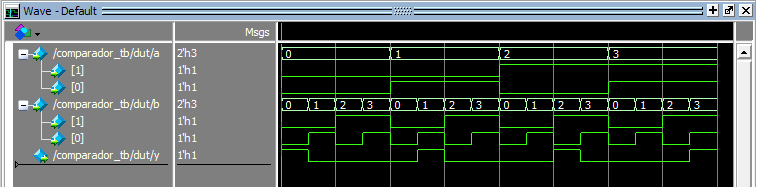
\includegraphics[width=1.0\textwidth]{comparador_wave.png}

\newpage

\section*{Atividade 3}
\setcounter{section}{3}
\setcounter{subsection}{0}

\subsection{Comparador Comportamental}
\begin{minted}{verilog}
module comparador2bits (
    input [1:0] a, b,
    output y
);

reg y_comp;

always @(*) begin
    if (a == b)
        y_comp = 1;
    else
        y_comp = 0;
end

assign y = y_comp;

endmodule
\end{minted}

\subsection{Console output}
\begin{verbatim}
a[1] | a[0] | b[1] | b[0] | y
   0 |    0 |    0 |    0 | 1
   0 |    0 |    0 |    1 | 0
   0 |    0 |    1 |    0 | 0
   0 |    0 |    1 |    1 | 0
   0 |    1 |    0 |    0 | 0
   0 |    1 |    0 |    1 | 1
   0 |    1 |    1 |    0 | 0
   0 |    1 |    1 |    1 | 0
   1 |    0 |    0 |    0 | 0
   1 |    0 |    0 |    1 | 0
   1 |    0 |    1 |    0 | 1
   1 |    0 |    1 |    1 | 0
   1 |    1 |    0 |    0 | 0
   1 |    1 |    0 |    1 | 0
   1 |    1 |    1 |    0 | 0
   1 |    1 |    1 |    1 | 1
\end{verbatim}

\subsection{Comparador Comportamental - Portas lógicas}
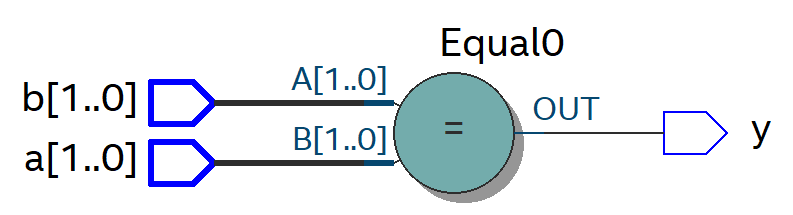
\includegraphics[width=1\textwidth]{comportamental_rtl.png}

\subsection{Comparador Comportamental - Simulação}
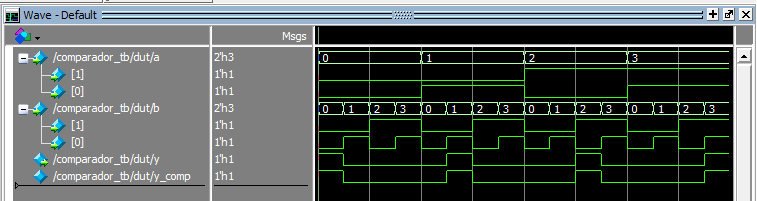
\includegraphics[width=1\textwidth]{comportamental_wave.png}

\end{document}
